\documentclass[serif]{beamer}\usepackage[]{graphicx}\usepackage[]{color}
%% maxwidth is the original width if it is less than linewidth
%% otherwise use linewidth (to make sure the graphics do not exceed the margin)
\makeatletter
\def\maxwidth{ %
  \ifdim\Gin@nat@width>\linewidth
    \linewidth
  \else
    \Gin@nat@width
  \fi
}
\makeatother

\definecolor{fgcolor}{rgb}{0.345, 0.345, 0.345}
\newcommand{\hlnum}[1]{\textcolor[rgb]{0.686,0.059,0.569}{#1}}%
\newcommand{\hlstr}[1]{\textcolor[rgb]{0.192,0.494,0.8}{#1}}%
\newcommand{\hlcom}[1]{\textcolor[rgb]{0.678,0.584,0.686}{\textit{#1}}}%
\newcommand{\hlopt}[1]{\textcolor[rgb]{0,0,0}{#1}}%
\newcommand{\hlstd}[1]{\textcolor[rgb]{0.345,0.345,0.345}{#1}}%
\newcommand{\hlkwa}[1]{\textcolor[rgb]{0.161,0.373,0.58}{\textbf{#1}}}%
\newcommand{\hlkwb}[1]{\textcolor[rgb]{0.69,0.353,0.396}{#1}}%
\newcommand{\hlkwc}[1]{\textcolor[rgb]{0.333,0.667,0.333}{#1}}%
\newcommand{\hlkwd}[1]{\textcolor[rgb]{0.737,0.353,0.396}{\textbf{#1}}}%

\usepackage{framed}
\makeatletter
\newenvironment{kframe}{%
 \def\at@end@of@kframe{}%
 \ifinner\ifhmode%
  \def\at@end@of@kframe{\end{minipage}}%
  \begin{minipage}{\columnwidth}%
 \fi\fi%
 \def\FrameCommand##1{\hskip\@totalleftmargin \hskip-\fboxsep
 \colorbox{shadecolor}{##1}\hskip-\fboxsep
     % There is no \\@totalrightmargin, so:
     \hskip-\linewidth \hskip-\@totalleftmargin \hskip\columnwidth}%
 \MakeFramed {\advance\hsize-\width
   \@totalleftmargin\z@ \linewidth\hsize
   \@setminipage}}%
 {\par\unskip\endMakeFramed%
 \at@end@of@kframe}
\makeatother

\definecolor{shadecolor}{rgb}{.97, .97, .97}
\definecolor{messagecolor}{rgb}{0, 0, 0}
\definecolor{warningcolor}{rgb}{1, 0, 1}
\definecolor{errorcolor}{rgb}{1, 0, 0}
\newenvironment{knitrout}{}{} % an empty environment to be redefined in TeX

\usepackage{alltt}
\usetheme{Boadilla}
\usepackage{graphicx}
\usepackage[final]{animate}
\usepackage{breqn}
\usepackage{xcolor}
\usepackage{booktabs}
\usepackage{tikz}
\usetikzlibrary{decorations.pathreplacing}
\usetikzlibrary{shapes,arrows,positioning,shadows}
\definecolor{links}{HTML}{2A1B81}
\hypersetup{colorlinks,linkcolor=links,urlcolor=links}
\usepackage{subfig}
\usepackage{pgf}
\usepackage{pgffor}

% knitr and global options


% load R libraries


\setbeamerfont{title}{series = \bfseries}
\setbeamerfont{frametitle}{series = \bfseries} 

\newcommand{\Bigtxt}[1]{\textbf{\textit{#1}}}
\IfFileExists{upquote.sty}{\usepackage{upquote}}{}
\begin{document}

\title[Comparison of WRTDS and GAMs]{Comparison of WRTDS and GAMs for evaluating long-term trends in chlorophyll}

\author[Beck, Murphy]{Marcus W. Beck\inst{1} \and Rebecca Murphy\inst{2}}

\date{October 16, 2015}

\institute[]{\inst{1} ORISE, USEPA, Gulf Ecology Division, \href{mailto:beck.marcus@epa.gov}{beck.marcus@epa.gov} \and \inst{2} UMCES at Chesapeake Bay Program, \href{mailto:rmurphy@chesapeakebay.net}{rmurphy@chesapeakebay.net}}

%%%%%%
\begin{frame}
\titlepage
\end{frame}

%%%%%%
\begin{frame}{Since the last call...}
\begin{itemize}
\item Application of GAMs and WRTDS to 30 year time series of monthly chlorophyll at LE1.2 and TF1.6 \\~\\
\item Development of comparable methods for model fitting \\~\\
\item Development of simulated datasets to evaluate flow-normalization \\~\\
\item Comparison of results and conclusions
\end{itemize}
\end{frame}

%%%%%%
\begin{frame}{Model applications}
Both models used Vertically-integrated chlorophyll, monthly timestep \\~\\
LE1.2: lnchla $\sim$ time + \Bigtxt{salinity} \\~\\
TF1.6: lnchla $\sim$ time + \Bigtxt{flow} \\~\\
Fits evaluated for whole time series and annual/seasonal/flow aggregations: \\~\\
\begin{itemize}
\item predicted to observed, GAM predicted to WRTDS predicted
\item Trends in flow-normalized results (average and \% change overall, by time period)
\end{itemize}
\end{frame}

%%%%%%
\begin{frame}{Model applications}
For comparing each model's \Bigtxt{predictions to observed}, at both sites:\\~\\
\begin{center}
$RMSE_{fit} = \sqrt {\frac{{\sum\limits_{{i = 1}}^n {{{\left( {{Chl_i} - {\widehat{Chl}_i}} \right)}^2}} }}{n}}$
\end{center}
For comparing \Bigtxt{predictions between models}, at both sites: \\~\\
\begin{center} 
$RMSE_{btw} = \sqrt {\frac{{\sum\limits_{{i = 1}}^n {{{\left( {{\widehat{Chl}_{WRTDS,\,i}} - {{\widehat{Chl}}_{GAM,\,i}}} \right)}^2}} }}{n}}$
\end{center}
\begin{center}
$\textrm{Average difference} = \left(\frac{\sum\limits_{i = 1}^n \widehat{Chl}_{WRTDS,\,i} - \sum\limits_{i = 1}^n \widehat{Chl}_{GAM,\,i}}{\sum\limits_{i = 1}^n \widehat{Chl}_{GAM,\,i}}\right) * 100$
\end{center}
\end{frame}

%%%%%%
\begin{frame}{Model fitting and flow-normalization}
\Bigtxt{Objective}: compare model fits \\~\\
\Bigtxt{Problem}: Need methods to prevent over-fitting and to compare apples-to-apples\\~\\
GAMs - identify optimal degrees of freedom for smoothing parameters \\~\\
WRTDS - identify optimal window widths for time, discharge (salinity or flow), and season \\~\\
Existing method for GAMs, k-fold cross-validation and search algorithm (`limited memory BFGS quasi-Newton method') to identify window-widths for WRTDS \\~\\
Basically, a statistical infrastructure to `automatically' fit the best model given the dataset \\~\\
\end{frame}

%%%%%%
\begin{frame}{Development of simulated datasets}
\Bigtxt{Objective}: evaluate ability of each model to reproduce flow-normalized trends\\~\\
\Bigtxt{Problem}: The true flow-normalized trends are not known and can only be empirically estimated \\~\\
We created monthly simulated datasets following the general technique in Hirsch et al. 2015 (sec. 4, MC simulations) \\
\begin{itemize}
\item Actual daily time series: discharge from Bowie gage, Jug Bay fluorescence
\item Overall: $Chl_{obs} = Chl_{flo} + Chl_{bio}$
\item From discharge: $Chl_{flo} = I\left(\widehat{Q}_{seas} + \sigma\cdot\varepsilon_{Q,\,sim}\right)$
\item From fluorescence: $Chl_{bio} = \widehat{Chl}_{seas} + \sigma\cdot\varepsilon_{Chl,\,sim}$
\item indicator $I$ changes to simulate changing flow component
\end{itemize}
\end{frame}

%%%%%%
\begin{frame}[fragile]{Development of simulated datasets}
\begin{knitrout}
\definecolor{shadecolor}{rgb}{0.929, 0.973, 0.984}\color{fgcolor}

{\centering 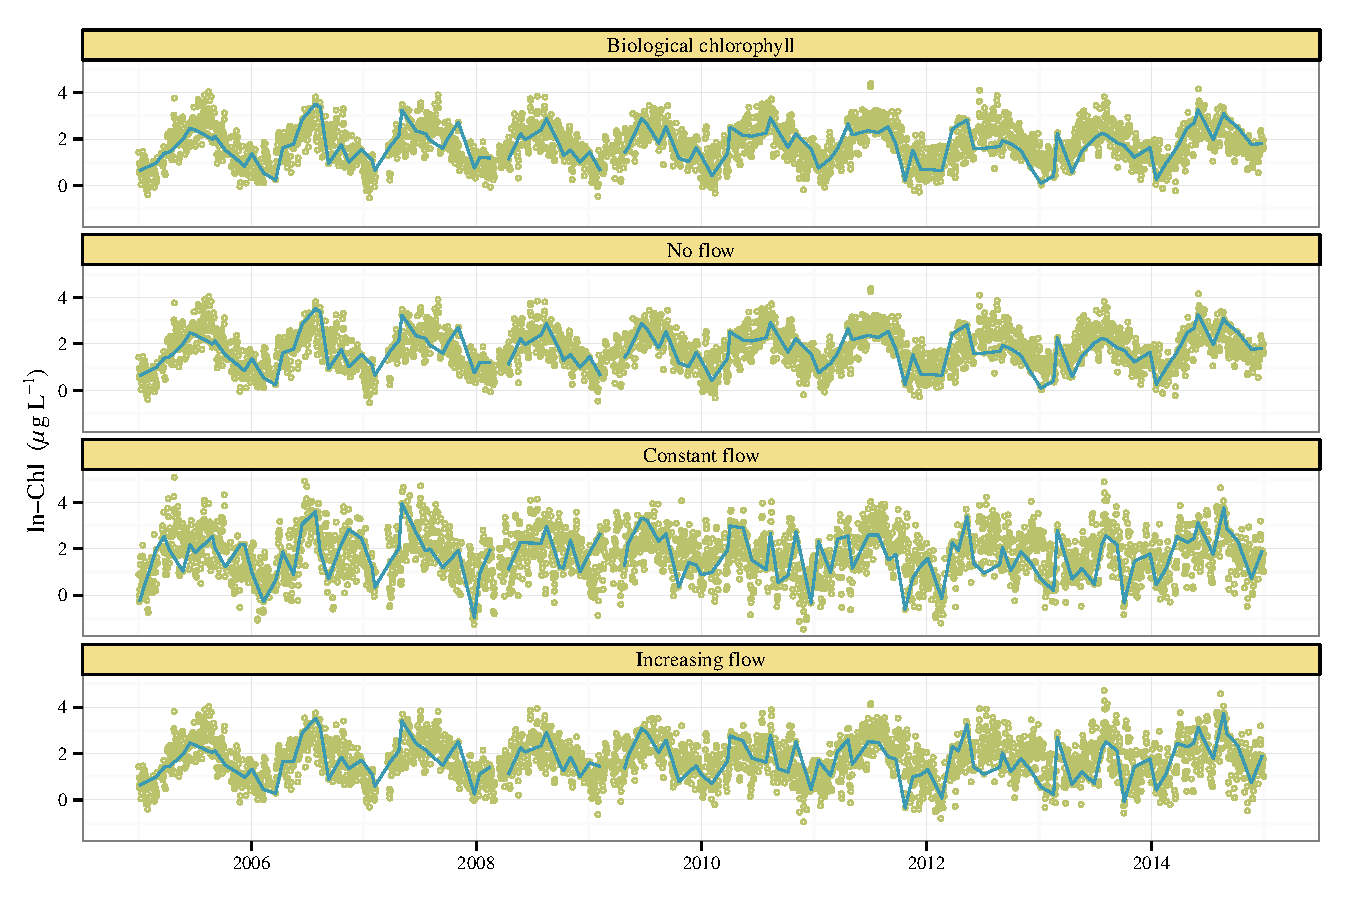
\includegraphics[width=\maxwidth]{figs/unnamed-chunk-2-1} 

}



\end{knitrout}
\end{frame}



%%%%%%
\begin{frame}{Results}
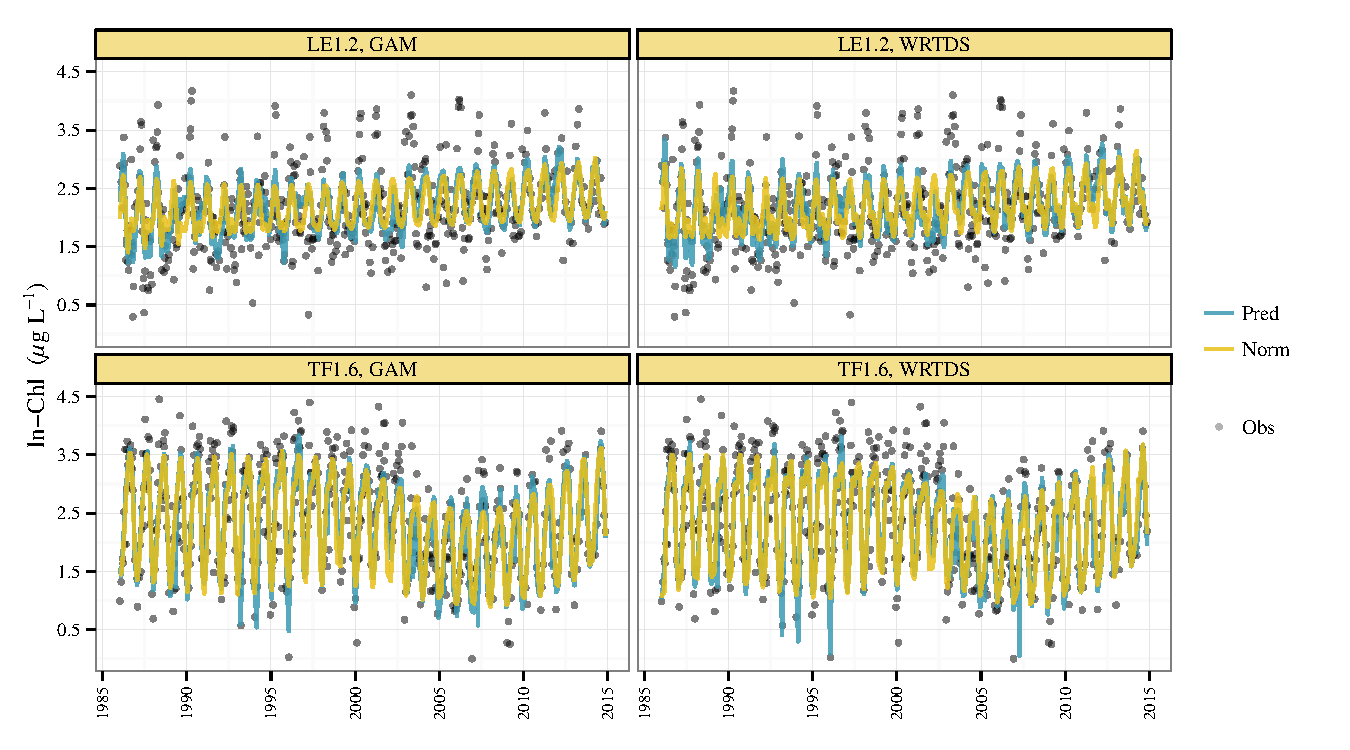
\includegraphics[width=\textwidth]{figs/predmo.pdf}
\end{frame}

%%%%%%
\begin{frame}{Results}
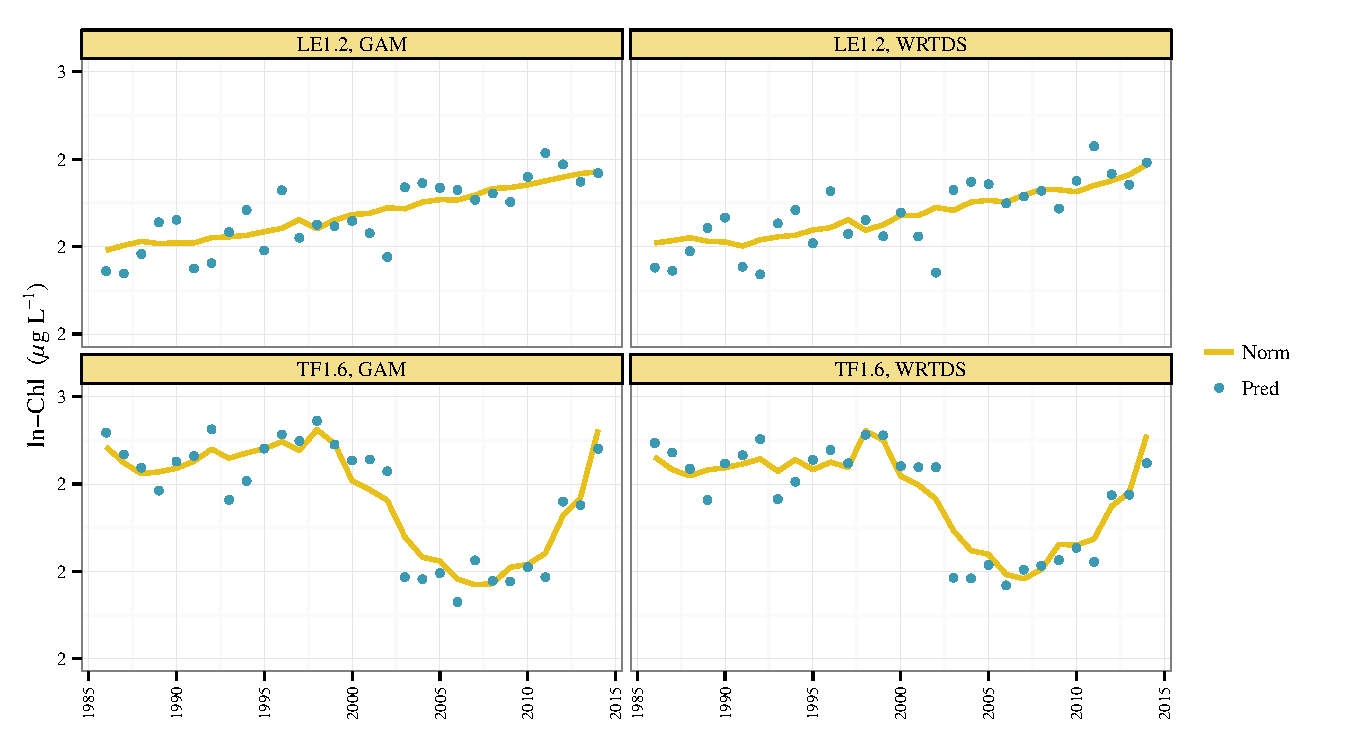
\includegraphics[width=\textwidth]{figs/predann.pdf}
\end{frame}

%%%%%%
\begin{frame}{Results}
\scriptsize
%latex.default(tab, file = "", rowlabel = "Period", caption = cap.val,     caption.loc = "top", rgroup = c("All", "Annual", "Seasonal",         "Flow"), n.rgroup = c(1, rep(4, 3)), cgroup = c("LE1.2",         "TF1.6"), n.cgroup = c(2, 2), rowname = rows, colheads = rep(c("GAM",         "WRTDS"), 2), label = "tab:perftoobs")%
\begin{table}[!tbp]
\caption{RMSE of observed to predicted ln-chlorophyll.\label{tab:perftoobs}} 
\begin{center}
\begin{tabular}{lllcll}
\hline\hline
\multicolumn{1}{l}{\bfseries Period}&\multicolumn{2}{c}{\bfseries LE1.2}&\multicolumn{1}{c}{\bfseries }&\multicolumn{2}{c}{\bfseries TF1.6}\tabularnewline
\cline{2-3} \cline{5-6}
\multicolumn{1}{l}{}&\multicolumn{1}{c}{GAM}&\multicolumn{1}{c}{WRTDS}&\multicolumn{1}{c}{}&\multicolumn{1}{c}{GAM}&\multicolumn{1}{c}{WRTDS}\tabularnewline
\hline
{\bfseries All}&&&&&\tabularnewline
~~&0.54&0.51&&0.54&0.52\tabularnewline
\hline
{\bfseries Annual}&&&&&\tabularnewline
~~1986-1993&0.54&0.50&&0.53&0.49\tabularnewline
~~1994-2000&0.52&0.50&&0.58&0.58\tabularnewline
~~2001-2007&0.63&0.60&&0.54&0.53\tabularnewline
~~2008-2014&0.39&0.36&&0.49&0.44\tabularnewline
\hline
{\bfseries Seasonal}&&&&&\tabularnewline
~~JFM&0.61&0.58&&0.53&0.49\tabularnewline
~~AMJ&0.69&0.64&&0.60&0.58\tabularnewline
~~JAS&0.38&0.35&&0.48&0.46\tabularnewline
~~OND&0.41&0.38&&0.55&0.54\tabularnewline
\hline
{\bfseries Flow}&&&&&\tabularnewline
~~1 (Low)&0.40&0.36&&0.48&0.46\tabularnewline
~~2&0.47&0.42&&0.56&0.54\tabularnewline
~~3&0.61&0.57&&0.56&0.52\tabularnewline
~~4 (High)&0.64&0.63&&0.56&0.54\tabularnewline
\hline
\end{tabular}\end{center}

\end{table}

\end{frame}

%%%%%%
\begin{frame}{Results}
\scriptsize
%latex.default(tab, file = "", rowlabel = "Period", caption = cap.val,     caption.loc = "top", rgroup = c("All", "Annual", "Seasonal",         "Flow"), n.rgroup = c(1, rep(4, 3)), cgroup = c("LE1.2",         "TF1.6"), n.cgroup = c(2, 2), rowname = rows, colheads = rep(c("Ave. diff.",         "RMSE"), 2), label = "tab:perfbtw")%
\begin{table}[!tbp]
\caption{Comparison of predicted results between models.\label{tab:perfbtw}} 
\begin{center}
\begin{tabular}{lllcll}
\hline\hline
\multicolumn{1}{l}{\bfseries Period}&\multicolumn{2}{c}{\bfseries LE1.2}&\multicolumn{1}{c}{\bfseries }&\multicolumn{2}{c}{\bfseries TF1.6}\tabularnewline
\cline{2-3} \cline{5-6}
\multicolumn{1}{l}{}&\multicolumn{1}{c}{Ave. diff.}&\multicolumn{1}{c}{RMSE}&\multicolumn{1}{c}{}&\multicolumn{1}{c}{Ave. diff.}&\multicolumn{1}{c}{RMSE}\tabularnewline
\hline
{\bfseries All}&&&&&\tabularnewline
~~&-0.11&0.15&& 0.01&0.17\tabularnewline
\hline
{\bfseries Annual}&&&&&\tabularnewline
~~1986-1993& 0.18&0.16&&-0.78&0.17\tabularnewline
~~1994-2000& 0.53&0.15&&-1.09&0.19\tabularnewline
~~2001-2007&-0.95&0.14&& 0.48&0.14\tabularnewline
~~2008-2014&-0.18&0.14&& 3.12&0.18\tabularnewline
\hline
{\bfseries Seasonal}&&&&&\tabularnewline
~~JFM& 2.91&0.14&&-5.02&0.22\tabularnewline
~~AMJ&-3.42&0.17&& 0.93&0.14\tabularnewline
~~JAS& 5.03&0.14&&-0.10&0.17\tabularnewline
~~OND&-5.25&0.14&& 2.08&0.17\tabularnewline
\hline
{\bfseries Flow}&&&&&\tabularnewline
~~Flow 1 (Low)& 0.19&0.16&&-0.09&0.12\tabularnewline
~~Flow 2&-0.83&0.16&& 0.73&0.15\tabularnewline
~~Flow 3& 0.19&0.15&& 0.84&0.20\tabularnewline
~~Flow 4 (High)& 0.03&0.13&&-1.62&0.20\tabularnewline
\hline
\end{tabular}\end{center}

\end{table}

\end{frame}

%%%%%%
\begin{frame}{Results}
\begin{knitrout}
\definecolor{shadecolor}{rgb}{0.929, 0.973, 0.984}\color{fgcolor}\begin{figure}[!ht]

{\centering 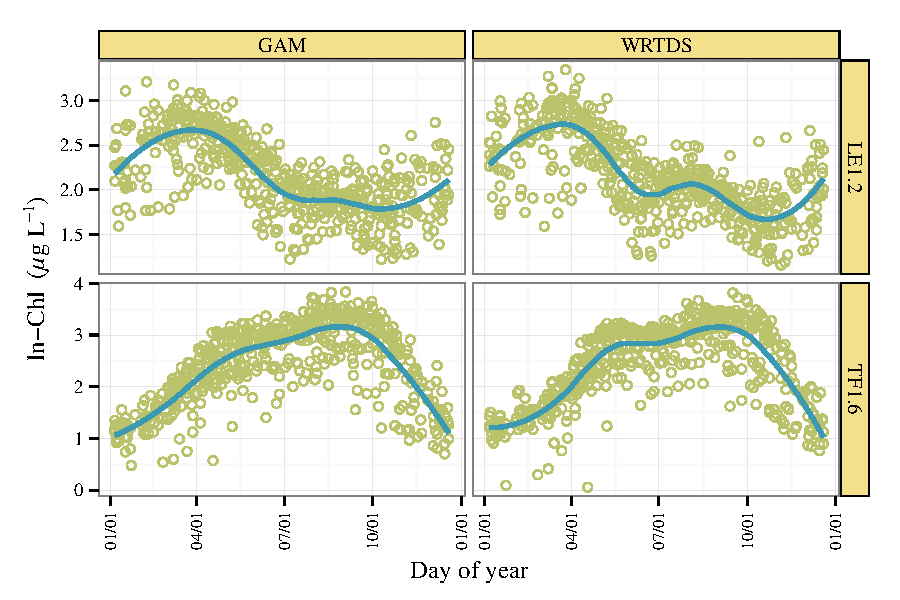
\includegraphics[width=0.9\textwidth]{figs/unnamed-chunk-6-1} 

}

\caption[Seasonal variation from model predictions]{Seasonal variation from model predictions.}\label{fig:unnamed-chunk-6}
\end{figure}


\end{knitrout}
\end{frame}



%%%%%%
\begin{frame}{Results}
\begin{figure}
\includegraphics<1>[width=\textwidth,page=2]{figs/dynaplots.pdf}
\includegraphics<2>[width=\textwidth,page=3]{figs/dynaplots.pdf}
\includegraphics<3>[width=\textwidth,page=4]{figs/dynaplots.pdf}
\includegraphics<4>[width=\textwidth,page=5]{figs/dynaplots.pdf}
\includegraphics<5>[width=\textwidth,page=6]{figs/dynaplots.pdf}
\includegraphics<6>[width=\textwidth,page=7]{figs/dynaplots.pdf}
\includegraphics<7>[width=\textwidth,page=8]{figs/dynaplots.pdf}
\includegraphics<8>[width=\textwidth,page=9]{figs/dynaplots.pdf}
\includegraphics<9>[width=\textwidth,page=10]{figs/dynaplots.pdf}
\includegraphics<10>[width=\textwidth,page=11]{figs/dynaplots.pdf}
\includegraphics<11>[width=\textwidth,page=12]{figs/dynaplots.pdf}
\includegraphics<12->[width=\textwidth,page=13]{figs/dynaplots.pdf}
\caption{Changes in the relationship between chlorophyll and flow across the time series, seaprate plots by month, model, and station.  The scales of salinity and flow are reversed for comparison of trends. Units are proportions of the total range in the observed data with values in each plot truncated by the monthly 5\textsuperscript{th} and 95\textsuperscript{th} percentiles.}
\end{figure}
\end{frame}

\end{document}
